%%PREAMBLE %%%%%%%%%%%%%%%%%%%%%%%%%%%%
\documentclass[10pt, a4paper]{article}% size of txt = 10pt
\usepackage[top= 2cm,
			bottom = 2cm,
			left = 1.7cm,
			right = 1.7cm,
			footskip = 0.5cm,
			headsep = 0cm,
			headheight = 0cm
					]{geometry}
\usepackage{amsmath} % math packages
\usepackage{amsfonts}% math packages
\usepackage{amssymb} % math packages
\usepackage{graphicx} %package for including graphics
\usepackage{array}
\usepackage[thinlines]{easytable}
\usepackage{float}
\usepackage[section]{placeins}
\usepackage[hidelinks]{hyperref}
\usepackage[shortlabels]{enumitem}
\usepackage{svg}
\usepackage{bigstrut}
\usepackage{wrapfig,lipsum,booktabs}
\usepackage{subcaption}
\usepackage{xfrac}
\usepackage{pdfpages}
\usepackage{listings}
\usepackage{xcolor}

\usepackage{listings}
\usepackage{color} %red, green, blue, yellow, cyan, magenta, black, white
\definecolor{mygreen}{RGB}{28,172,0} % color values Red, Green, Blue
\definecolor{mylilas}{RGB}{170,55,241}

\definecolor{codegreen}{rgb}{0,0.6,0}
\definecolor{codegray}{rgb}{0.5,0.5,0.5}
\definecolor{codepurple}{rgb}{0.58,0,0.82}
\definecolor{backcolour}{rgb}{1,1,1}

\lstdefinestyle{mystyle}{
    backgroundcolor=\color{backcolour},   
    commentstyle=\color{codegreen},
    keywordstyle=\color{magenta},
    numberstyle=\tiny\color{codegray},
    stringstyle=\color{codepurple},
    basicstyle=\ttfamily\footnotesize,
    breakatwhitespace=false,         
    breaklines=true,                 
    captionpos=b,                    
    keepspaces=true,                 
    numbers=left,                    
    numbersep=5pt,                  
    showspaces=false,                
    showstringspaces=false,
    showtabs=false,                  
    tabsize=2
}
\lstset{style=mystyle}


%date format
\def\mydate{\leavevmode\hbox{\twodigits\day.\twodigits\month.\the\year}}
\def\twodigits#1{\ifnum#1<10 0\fi\the#1}


\usepackage[T1]{fontenc} 
\usepackage{lmodern}
\usepackage{indentfirst}
\setlength{\parindent}{1cm}

\makeatletter
\newcommand{\thickhline}{%
    \noalign {\ifnum 0=`}\fi \hrule height 2pt
    \futurelet \reserved@a \@xhline
}
\newcolumntype{"}{@{\hskip\tabcolsep\vrule width 2pt\hskip\tabcolsep}}
\makeatother
\newcolumntype{?}{!{\vrule width 2pt}}
%%DOC ENVIROMENT%%%%%%%%%%%%%%%%%%%%%%%
\begin{document}
%Title 
\begin{flushleft}%% left justification
	\textbf{\Large{MKC-KBC: Úkol č. 5}}\hfill Filip Paul\\
	\large{Bow-tie dipole a CPW \hfill\mydate}
\end{flushleft}

\section{\Large 3D modely zkoumaných scénářů s vyzařovací charakteristikou:}
\begin{figure}[ht!]
	\centering
	\begin{minipage}{0.32\textwidth}
		\centering
		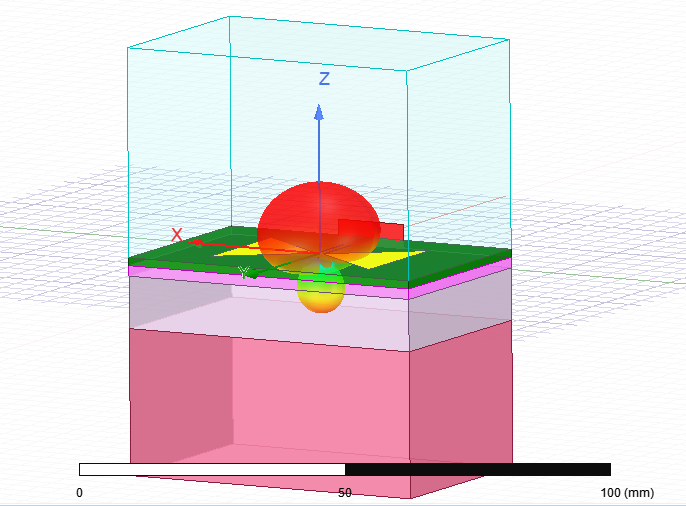
\includegraphics[width= 1\textwidth, height = 0.25\textheight]{3D_model.png}
		\captionof{figure}{3D: Bow-tie dipole}
	\end{minipage}%
	\hfill
	\begin{minipage}{0.32\textwidth}
		\centering
		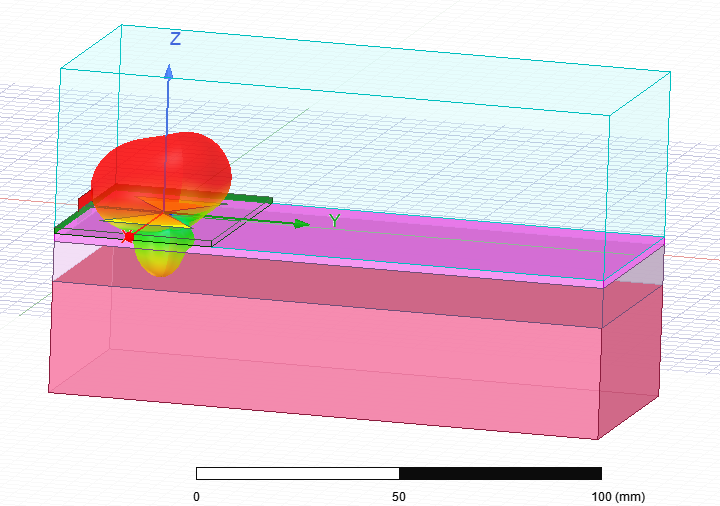
\includegraphics[width= 1\textwidth,height = 0.25\textheight]{3D_model_long.png}
		\captionof{figure}{3D: Bow-tie dipole - propagation}
	\end{minipage}
	\hfill
	\begin{minipage}{0.32\textwidth}
		\centering
		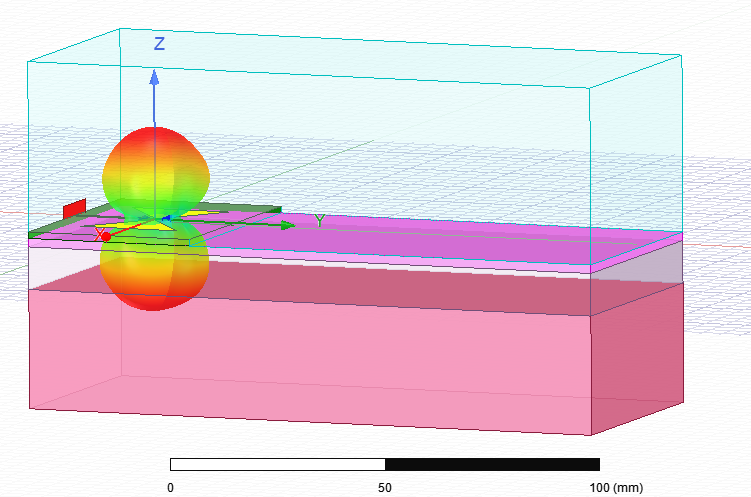
\includegraphics[width= 1\textwidth,height = 0.25\textheight]{3D_model_GHz.png}
		\captionof{figure}{3D: Free space}
	\end{minipage}
	\end{figure}

	\begin{figure}[ht!]
		\centering
		\begin{minipage}{0.32\textwidth}
			\centering
			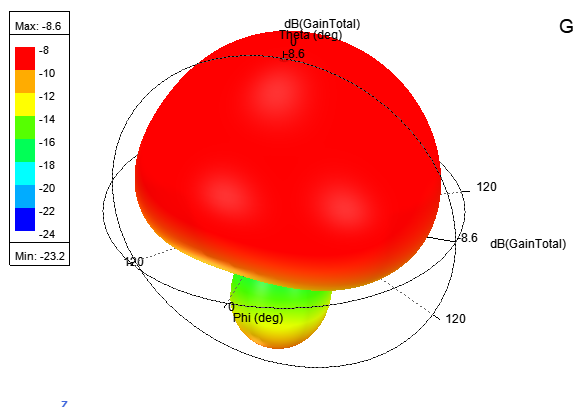
\includegraphics[width = 1\textwidth]{GAIN_model.png}
			\captionof{figure}{Vyz. char: Bow-tie dipole}
		\end{minipage}%
		\hfill
		\begin{minipage}{0.32\textwidth}
			\centering
			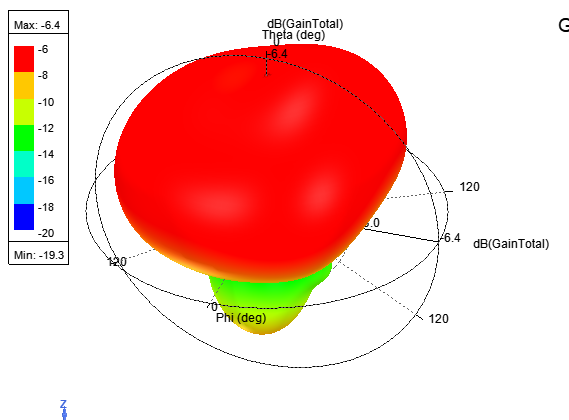
\includegraphics[width= 1\textwidth]{GAIN_model_long.png}
			\captionof{figure}{Vyz. char: Bow-tie dipole - propagation}
		\end{minipage}
		\hfill
		\begin{minipage}{0.32\textwidth}
			\centering
			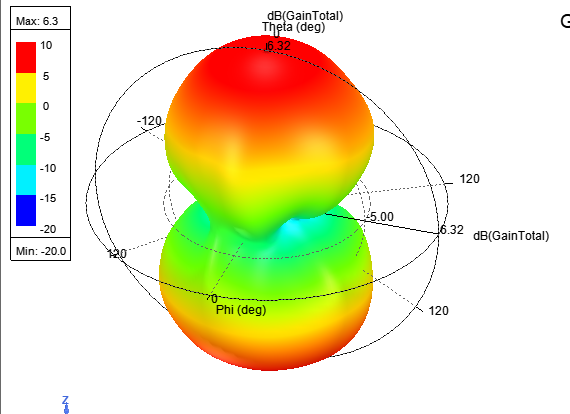
\includegraphics[width= 1\textwidth]{GAIN_model_GHz.png}
			\captionof{figure}{Vyz. char: Free space}
		\end{minipage}
		\end{figure}


		Z vyzařovacích charakteristik je patrné, že přiložený fantom má poměrně značný vliv.
		Fantom má totiž oproti vakuu nenulové ztráty a značnou vodivost. Což vede jednak k odrazům
		tak ke ztrátě (přeměně) energie. Vyzařovací charakteristiky pro Obr. 4 a 5 jsou simulovány
		pro 2.45GHz. Charakteristika z obrázku 6 je simulována pro 6GHz, což je přibližná hodnota
		rezonančního kmitočtu ve vakuu.
		\clearpage
	\section{\Large Impedanční přizpůsobení antény a CPW}

	\begin{figure}[ht!]
		\centering
		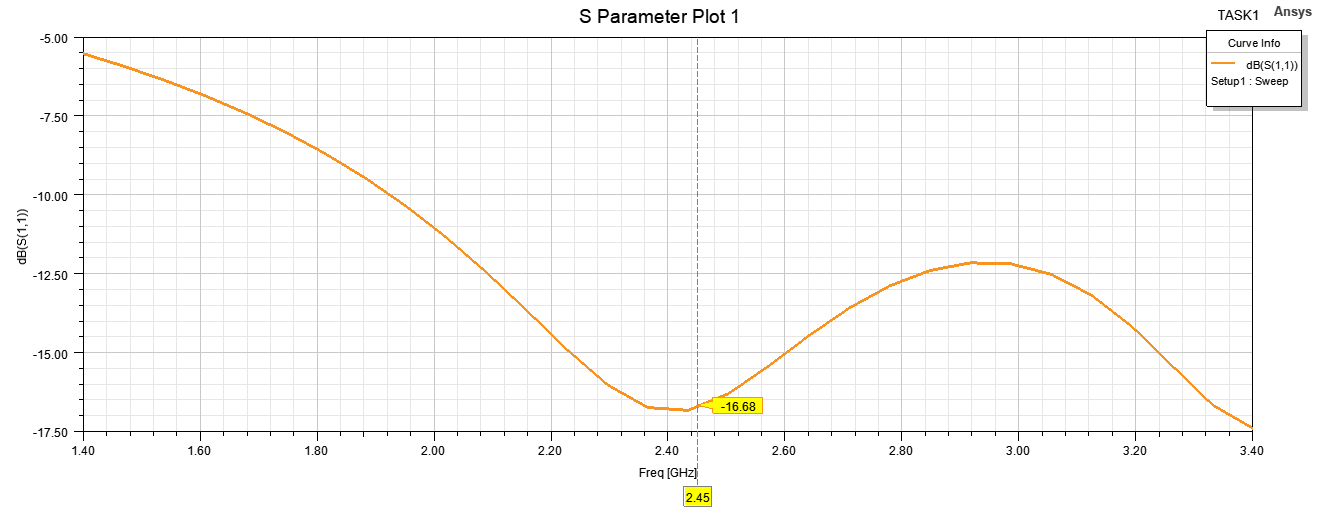
\includegraphics[width = 1\textwidth]{S11.png}
		\captionof{figure}{S11 parametry pro model (obr.1)}
	\end{figure}

	\begin{figure}[ht!]
		\centering
		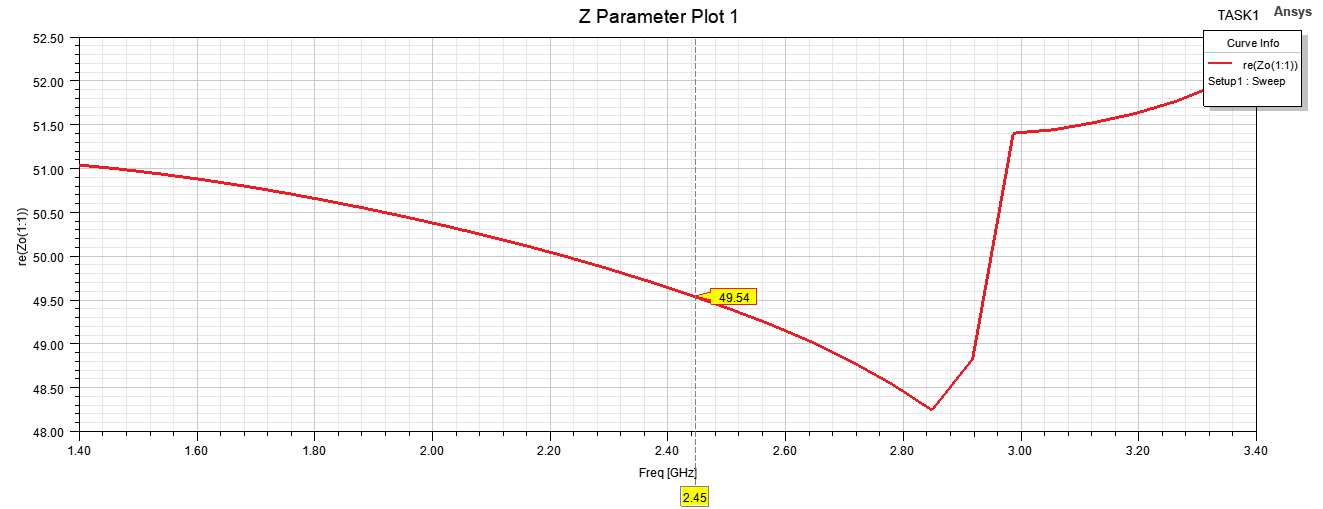
\includegraphics[width = 1\textwidth]{char_imp.png}
		\captionof{figure}{char impedance CPW pro model (obr.1)}
	\end{figure}

	Z hodnot S11 parametrů kmitočet okolo 2.43\,GHz. Impedance
	CPW se blíží k 50\,Ohmům, což značí dobré přizpůsobení.
	\clearpage
	\section{\Large Propagace záření ve směru Y}
	
	\begin{figure}[ht!]
		\centering
		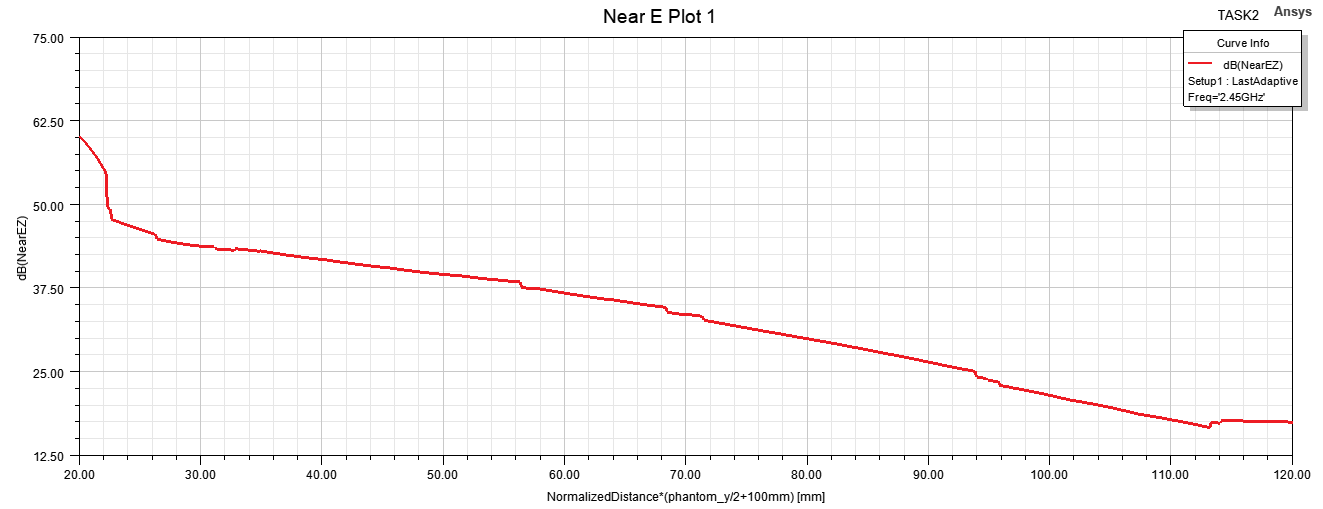
\includegraphics[width = 1\textwidth]{Z_near.png}
		\captionof{figure}{Ez složka v blízkém poli pro model (obr.2)}
	\end{figure}
	Z obrázku 9 je patrné, že intenzita pole E ve směru Y klesá. Výsledná křivka
	zobrazená v dB připomíná přímku, což v lineárních jednotkách odpovídá exponenciálnímu
	poklesu intenzity. 

	\section{\Large Rezonance ve vakuu}
	Rezonanční kmitočet ve vakuu je přibližně 6\,GHz. Vyzařovací charatkteristika je zobrazena na obr. 6.
	\begin{figure}[ht!]
		\centering
		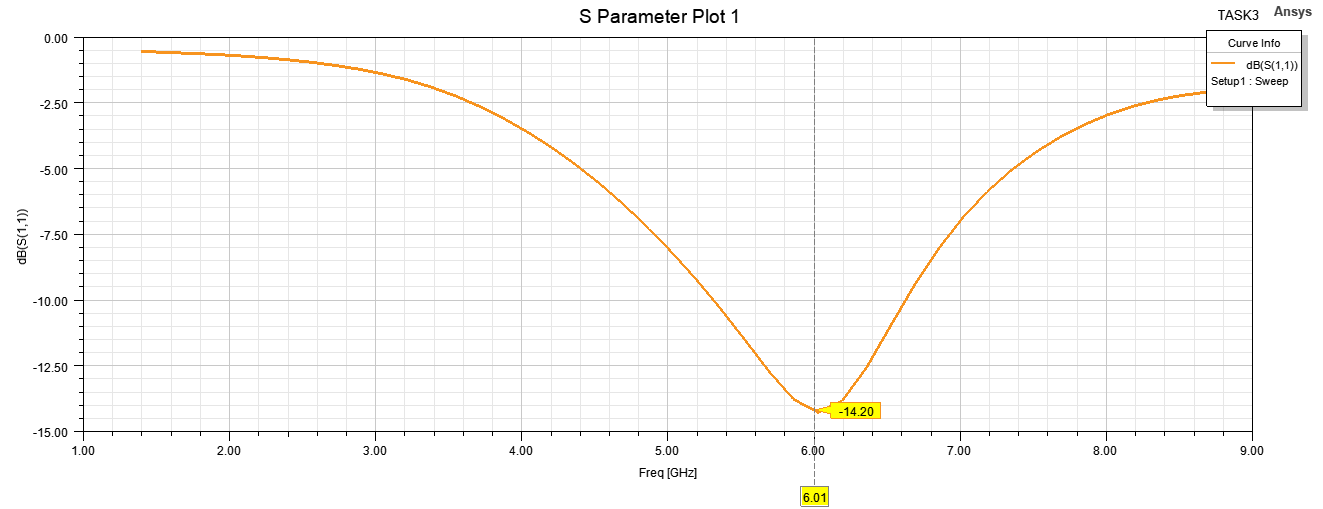
\includegraphics[width = 1\textwidth]{S11_freespace.png}
		\captionof{figure}{S11 parametr pro model (obr.3) - freespace}
	\end{figure}
\clearpage
\section{\Large Parametry použité v simulaci:}
	\begin{figure}[ht!]
		\centering
		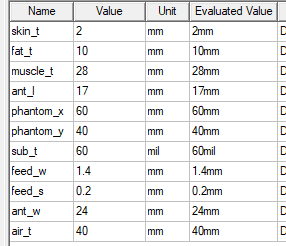
\includegraphics[]{global_variables.png}
		\captionof{figure}{Simulační proměnné}
	\end{figure}



\end{document}

%\[f(x)= (x+2)^2 - \frac{9\cdot 2\pi}{26}\] %%mathematic equatation in display style mode
%%optional:
%	\begin{align} %%this alignes all charakters after & if *is removed equations will be numbered
%	\hspace{5cm}  
%		 x &= a_2 x^2 +_1 x + a_0 \\
% 		x &=x^2 \nonumber		%no number will not add number to eq
%	\end{align}
